\chapter{Progettazione dell'applicazione}
\section{Architettura}
L'applicativo è stato scritto in 'C\#' facendo uso di dotnet 7 e windows forms,
Il tool ORM scelto è stato ef Core il quale ha automaticamente tradotto le tabelle in classi e ha esposto i metodi utili a manipolare il db.
\section{Gestore Simulazione}
All'apertura compare una finestra che permette di impostare i parametri e gestire la Simulazione:
\begin{figure}[H]
     \centering
     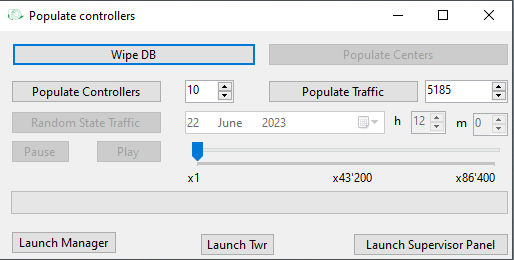
\includegraphics[width=1\textwidth]{figures/Sim.PNG}
     \caption{"La finestra per gestire la simulazione"}
   \end{figure}

\begin{itemize}
     \item WipeDb: Cancella tutti i dati della sessione precedente dal db.
     \item Populate Centers: Popula i centri, le posizioni, i settori e il numero minimo di controllori con le relative ferie.
     \item Populate Controllers: Genera Controllori aggiuntivi.
     \item Populate traffic: Genera il numero impostato di traffici nel mese corrente.
     \item Random state traffic: Posiziona ogni traffico nel punto della rotta che corrisponderebbe all'orario della simulazione ma con una variazione di orario dall'orario stimato con distribuzione normale (ma sbilanciata verso il ritardo)
     \item Pause, Play e lo slider: Permettono di gestire la riproduzione della simulazione.
     \item I tasti sul fondo permettono di lanciare gli strumenti effettivi. 
\end{itemize}
\section{Manager}
Questo tool è diviso in diverse tab:
La prima permette di vedere i controllori presenti in un centro e calcola per ognuno i turni svolti e la compensazione totale.
\begin{figure}[H]
     \centering
     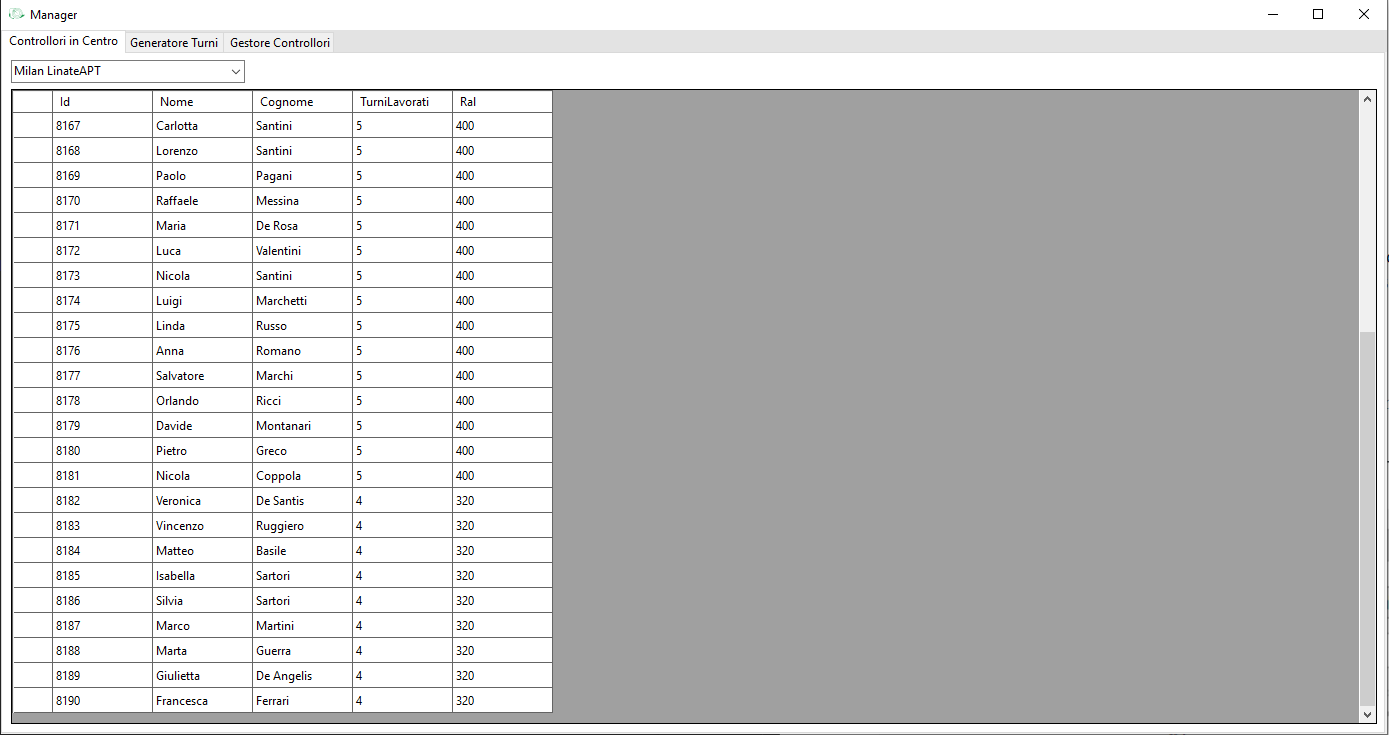
\includegraphics[width=1\textwidth]{figures/CIC.PNG}
     \caption{"La finestra che mostra i controllori in un centro"}
   \end{figure}
La seconda forse la più importante permette di generare i turni in un mese e di esportare la tabella.
   \begin{figure}[H]
        \centering
        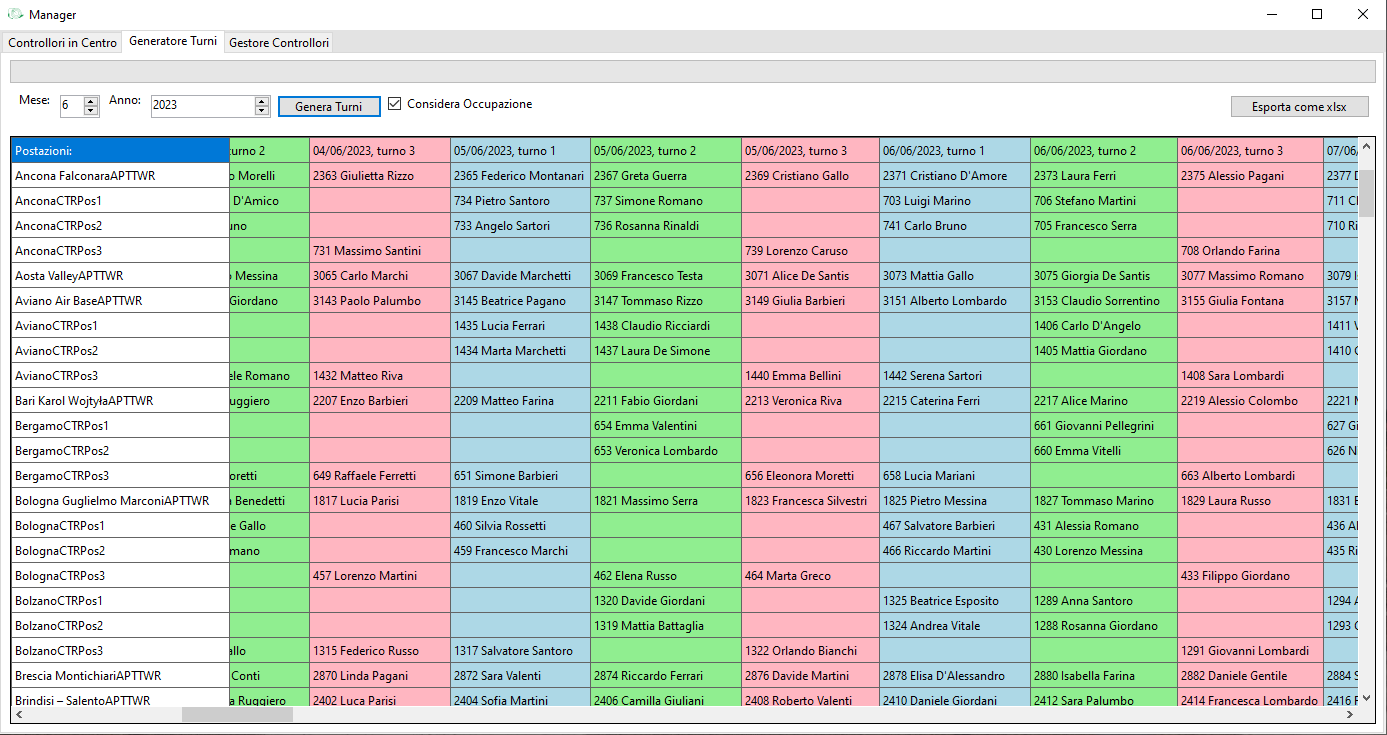
\includegraphics[width=1\textwidth]{figures/shifts.PNG}
        \caption{"La finestra che mostra i turni del mese"}
      \end{figure}
\pagebreak
La terza permette di gestire (Assumere, licenziare e modificare) i dati dei controllori e le loro ferie.
\begin{figure}[H]
     \centering
     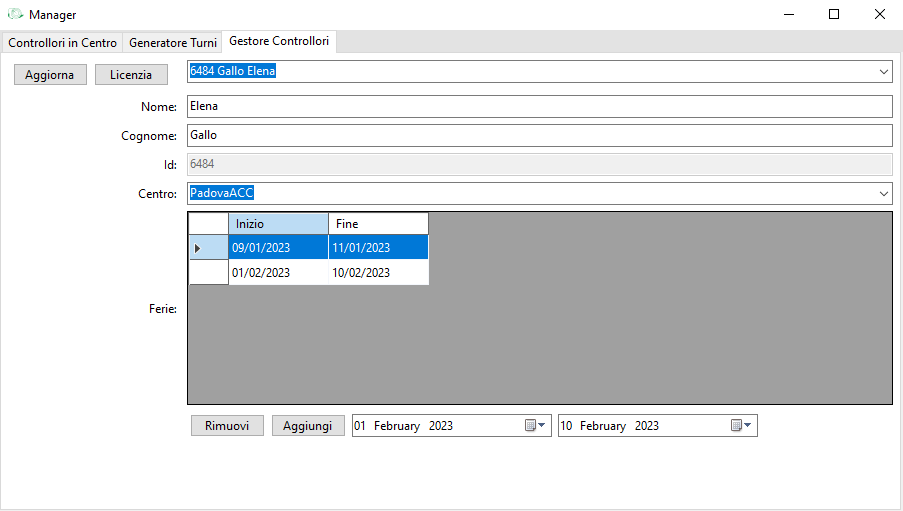
\includegraphics[width=1\textwidth]{figures/CM.PNG}
     \caption{"La finestra che gestisce i controllori"}
   \end{figure}
\pagebreak
\section{TWR Control}
Questo tool permette ad un controllore di svolgere il suo lavoro su una postazione di torre,
 selezionando l'A/D si ha hanno a disposizione i controllori abilitati e una volta effettuato il log in le tabelle di arrivi e partenze si popoleranno con i voli che sono prossimi all'arrivo o alla partenza permettendo al controllore di segnarne un cambio di stato quando questo avviene.
 \begin{figure}[H]
     \centering
     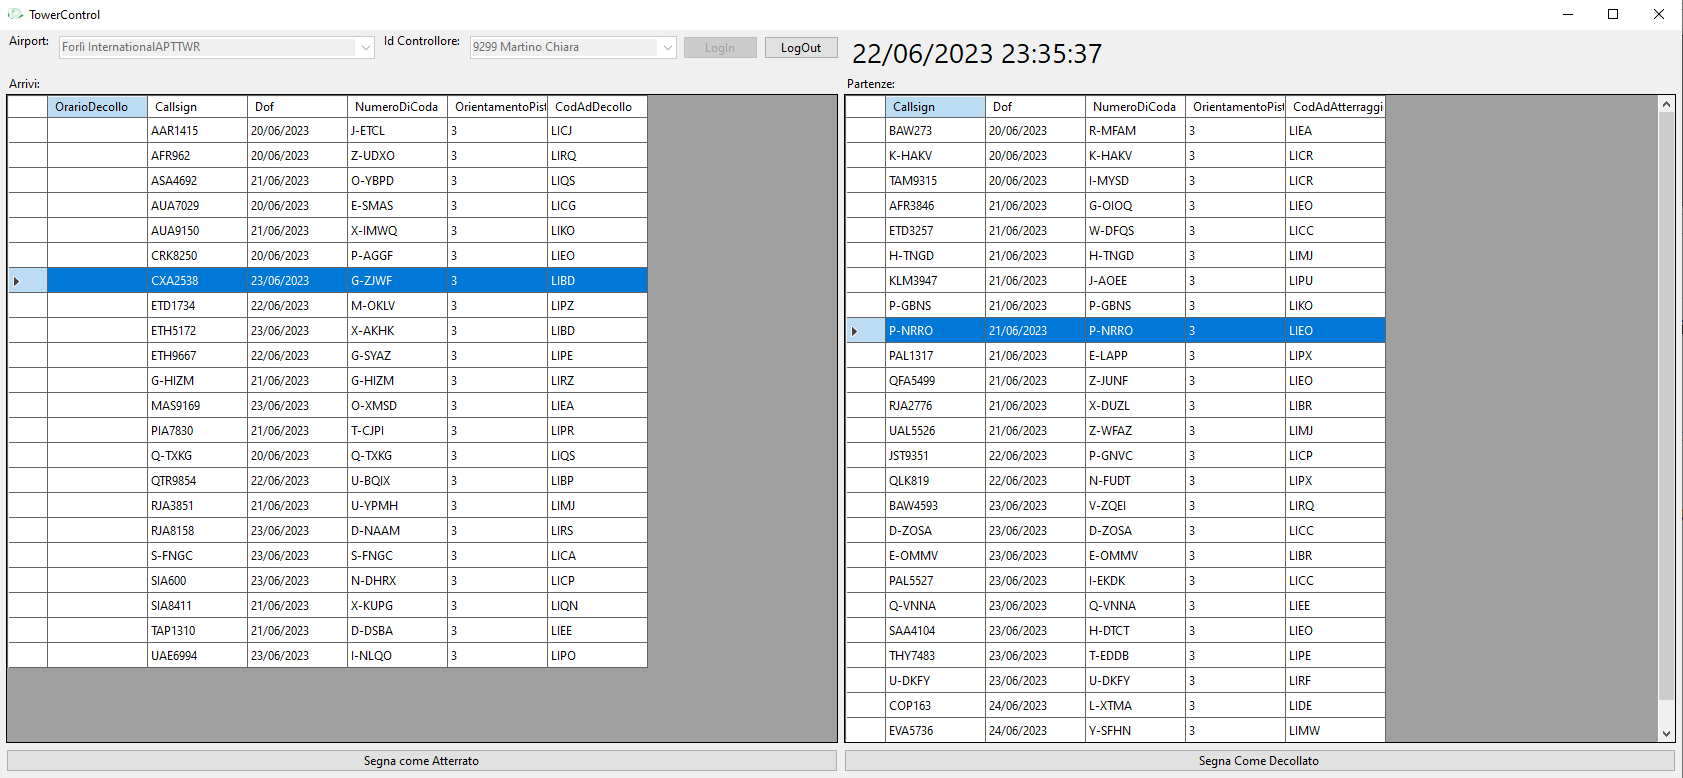
\includegraphics[width=1\textwidth]{figures/twr.PNG}
     \caption{"La finestra per gestire una posizione di torre"}
   \end{figure}
   \begin{figure}[H]
     \centering
     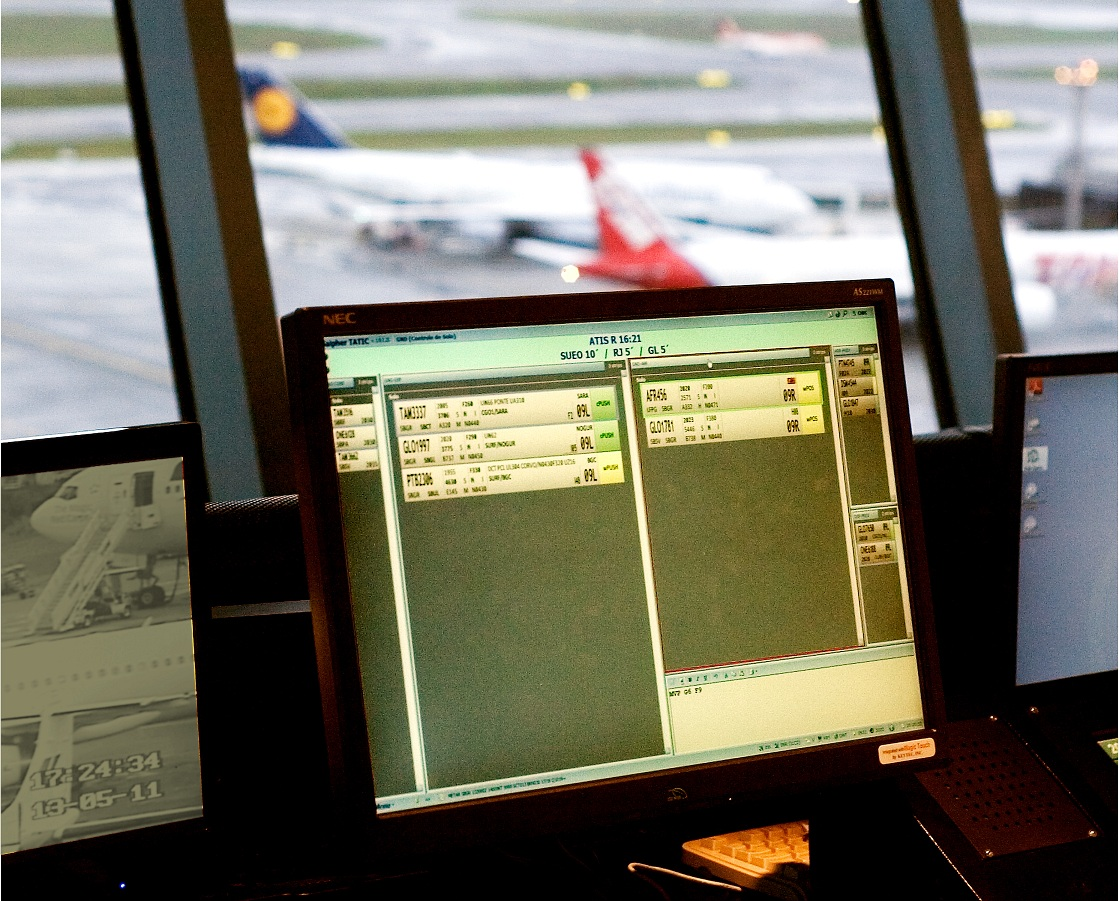
\includegraphics[width=12cm]{figures/TATIC_Electronic_Flight_Strip_system_at_Sao_Paulo_Itnl.jpg}
     \caption{"Un vero tool per gestire una posizione di torre Fonte: \url{https://commons.wikimedia.org/wiki/File:TATIC_Electronic_Flight_Strip_system_at_Sao_Paulo_Itnl.jpg}}
   \end{figure}
\section{Supervisor tool}
Questo strumento permette al supervisore di un centro di monitorare il traffico atteso nelle ore successive nelle posizioni del centro, in modo da prendere decisioni strategiche monitorando l'andamento del traffico.
è possibile aprire posizioni schierando i controllori in turno e anche quelli in turno stand by. La linea rossa sui grafici mostra la capacità massima del turno divisa per le ore.
\begin{figure}[H]
     \centering
     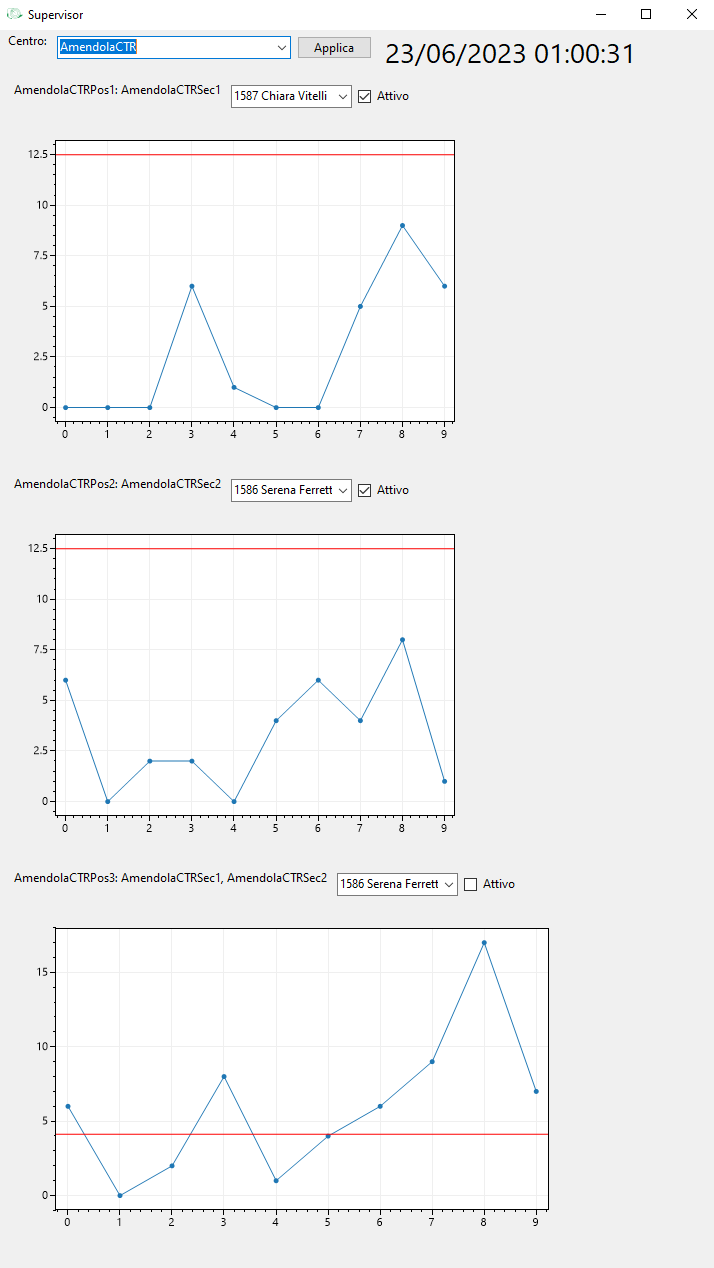
\includegraphics[height=19cm]{figures/sup.PNG}
     \caption{"La finestra del Supervisor tool"}
   \end{figure}
   \begin{figure}[H]
     \centering
     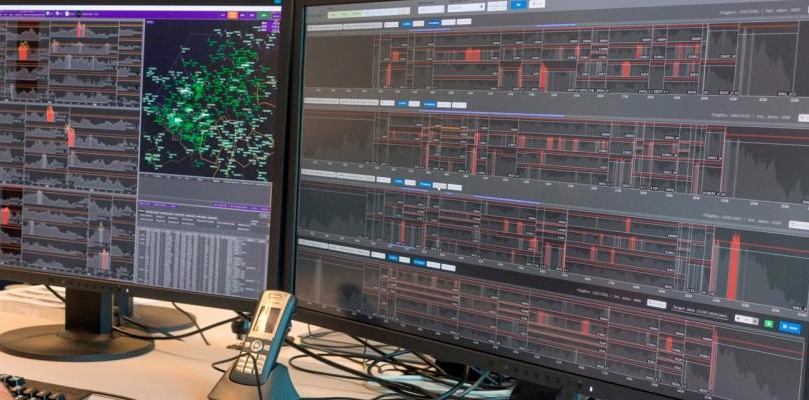
\includegraphics[width=1\textwidth]{figures/big-data-improve-capacity-planning-and-atm-efficiency_1.jpg}
     \caption{"Un vero tool di gestione dell'occupazione Fonte: \url{https://www.eurocontrol.int/press-release/big-data-improve-capacity-planning-and-atm-efficiency}}
   \end{figure}